\documentclass[a4paper, twocolumn, fleqn]{article}
\usepackage[english]{babel}
\usepackage{a4wide}

% Fonts
\usepackage[sc]{mathpazo}
\usepackage[T1]{fontenc}
\linespread{1.05}
\usepackage{lmodern}
\usepackage{microtype}
\usepackage{lettrine}

% Floats
\usepackage{float}
\usepackage[section]{placeins}

%Plaatjes
\usepackage{tikz}
\usepackage{graphicx}
\usepackage[small,labelfont=bf,up,textfont=sl,up]{caption}
\usepackage{subcaption}
\DeclareCaptionLabelFormat{opening}{(#2)}
\captionsetup{subrefformat=opening}


% Custom section headers
\usepackage{titlesec}
\titleformat{\section}[block]{\large\scshape}{\thesection.}{1em}{}
\titleformat{\subsubsection}[block]{\scshape}{\thesubsubsection.}{1em}{}

% References
\usepackage{varioref}
\usepackage{hyperref}
\usepackage[noabbrev]{cleveref}

% Plaatje boven titel
\usepackage{titling}

% References
\usepackage[backend=bibtex]{biblatex}

\usepackage{csquotes}
\bibliography{biblio}

% Temp
\usepackage[obeyFinal]{todonotes}

\predate{\centering\large}
\postdate{%
	\centering
	\vspace{2ex}
  	~\\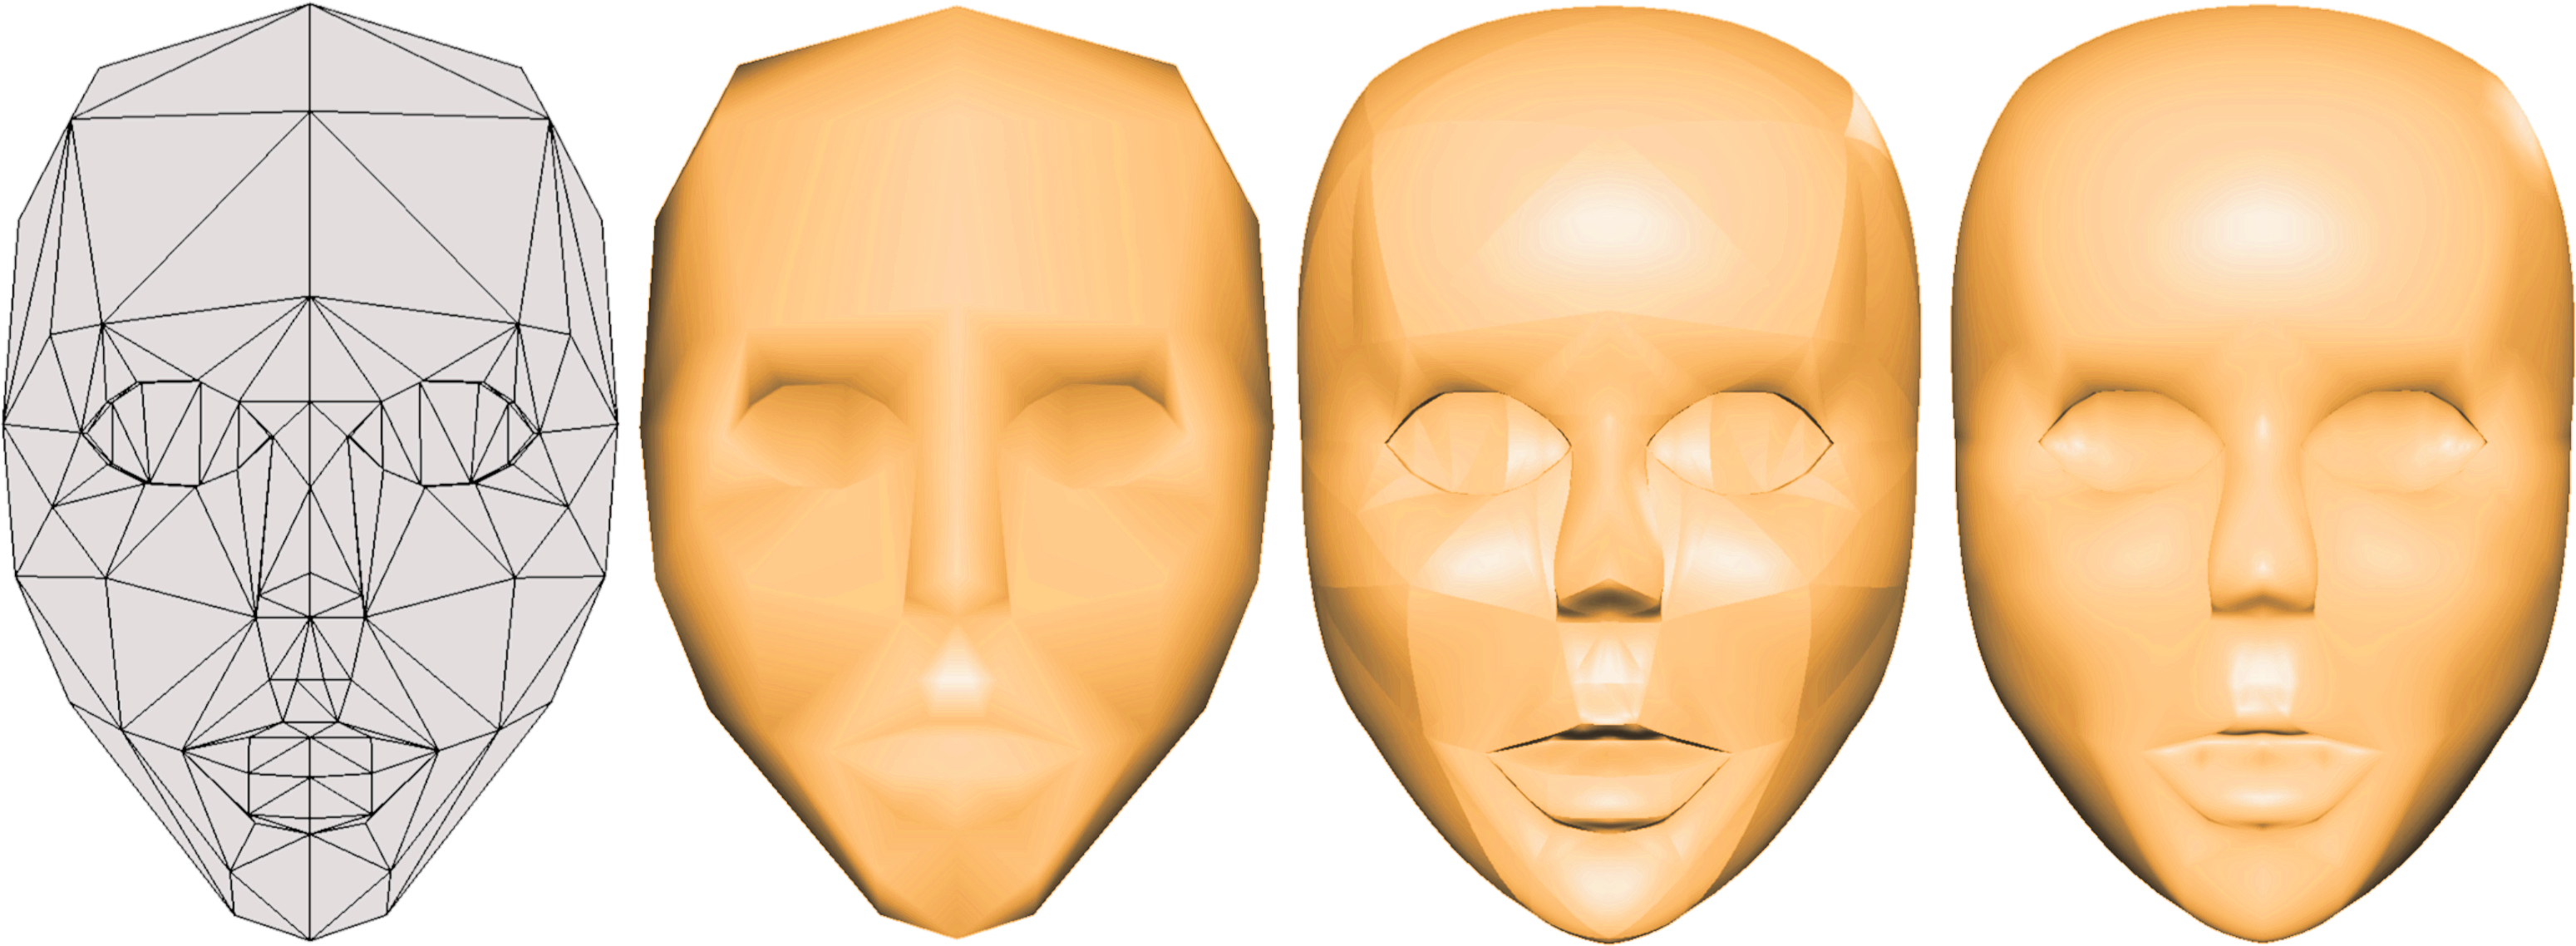
\includegraphics[width=0.9\textwidth]{img/plaatje.png}
  	\captionof{figure}{From left to right the input triangulation, the Gouraud shaded input triangulation, the geometric component of the PN triangles, shaded according to surface normal variation, and the curved PN triangles, shaded with independently constructed quadratically varying normals.}
  	\label{fig:sum:result}
}

\title{Curved PN Triangles}
\author{%
	Rick van Veen (s1883933)%
	%\thanks{These authors contributed equally to this work.}% 
	\and% 
	Laura Baakman (s1869140)%
	%\footnotemark[1]%
}

\begin{document}

\maketitle

%!TEX root = report.tex
\noindent Point normal triangles, or PN triangles for short, were introduced by \textcite{vlachos2001curved} to improve the visual quality of existing triangle-based art in real time entertainment. An important aspect of this approach is that it uses only the information of the primitive and not of adjacent triangles. Therefore no changes to authoring tools and hardware designs are needed while providing a smoother, although not everywhere tangent continuous, silhouette and more organic shapes, compare the two rightmost images in \cref{fig:sum:result}. We provide a brief review of the construction of a PN triangle mesh, its advantages and disadvantages, and where this approach fits in the graphics pipeline. 

\begin{figure*}
	\centering
	% \includegraphics[width=0.\textwidth]{./img/_}
	\missingfigure{Figure 1 from paper. This is the best single image we can provide, I guess.}
	\caption{From left to right (a) Input triangulation, (b) Gouraud shaded input triangulation, (c) geometric component of the PN triangles (shaded according to surface normal variation), and (d) curved PN Triangles (shaded with independently constructed quadratically varying normals)}
	\label{fig:sum:result}
\end{figure*}

A PN triangle is specified by its normal and geometric component. To capture inflections implied by these components at least a cubic geometry and quadratic normals are needed.

\subsubsection*{Geometry}
The geometry of a curved PN triangle is defined by a cubic b\'ezier patch. We can distinguish three sets of control points in such a patch: the vertex, tangent and center coefficients. Below we describe for each of these sets of control points how they are obtained from the input primitive. 

The vertex coefficients match the vertices of the input primitive. The tangent coefficients are the coefficients on the edge of the PN triangle that are not vertex coefficients. Initially the tangent coefficients are spread out uniformly over their associated edge. To obtain the final tangent coefficients, the initial coefficients are projected onto the tangent plane defined by the normal at the nearest vertex coefficient. 

The center vertex is the vertex in the center of the triangle. Its position is obtained by computing the average of the final tangent coefficients and raising it by the the difference between the tangent and vertex coefficients divided by two. We refer the reader to \textcite{vlachos2001curved} for the implementation details.

\subsubsection*{Normals}
A quadratic b\'ezier patch is used for the normal component of the PN triangles. To effectively capture inflections one needs to use quadratically varying normals. These normals are computed by reflecting the averaged vertex normals in the plane perpendicular to the edge placed at the middle of the edge.

The resulting mesh has $C^1$ continuity at the vertices and $C^0$ continuity everywhere else. 

\subsubsection*{Triangular Mesh}
Using the patch one can subdivide the primitives to a desired level of detail to generated a finer triangle mesh. 

One downside of PN triangle is that they cannot handle triangular patches that share vertices along a curved edge, but not normals at those vertices. The resulting triangulation will show cracks. One exception to this case is when the normals of a shared vertex are perpendicular to the edge. \citeauthor{vlachos2001curved} propose handling this case by using the information of adjacent triangles, we refer the reader to the original paper for the details.

% How does this fit in the pipeline
\subsubsection*{Graphics Pipeline}
It is important to note that at the time \textcite{vlachos2001curved} was published there were no programmable tesselation or geometry shader. The pipeline provided by \citeauthor{vlachos2001curved} suggests computing the PN-triangles in a preprocessing stage on the CPU. Today the full assembly of PN triangles could be done on the GPU by making use of tessellation shaders.\\



\printbibliography

\end{document}